\documentclass[11pt]{article}

\usepackage[portuguese]{babel}
\usepackage[utf8]{inputenc}
\usepackage{amsmath}
\usepackage{graphicx}
\usepackage{float}
\usepackage{subfig}
\usepackage{fixltx2e}
\usepackage[bottom]{footmisc}
\usepackage{listings}
\usepackage{color} 
\usepackage{xargs}                      % Use more than one optional parameter in a new commands
\usepackage[pdftex,dvipsnames]{xcolor}  % Coloured text etc.
\usepackage[colorinlistoftodos,prependcaption,textsize=tiny]{todonotes}
\newcommandx{\unsure}[2][1=]{\todo[linecolor=red,backgroundcolor=red!25,bordercolor=red,#1]{#2}}
\newcommandx{\change}[2][1=]{\todo[linecolor=blue,backgroundcolor=blue!25,bordercolor=blue,#1]{#2}}
\newcommandx{\info}[2][1=]{\todo[linecolor=OliveGreen,backgroundcolor=OliveGreen!25,bordercolor=OliveGreen,#1]{#2}}
\newcommandx{\improvement}[2][1=]{\todo[linecolor=Plum,backgroundcolor=Plum!25,bordercolor=Plum,#1]{#2}}
\newcommandx{\thiswillnotshow}[2][1=]{\todo[disable,#1]{#2}}
\usepackage[font=footnotesize]{caption}

\setcounter{tocdepth}{3}

\numberwithin{equation}{section}

\linespread{1.3}
\usepackage{indentfirst}
\usepackage[top=2cm, bottom=2cm, right=2.3cm, left=2.3cm]{geometry}
\addto\captionsportuguese{\renewcommand{\contentsname}{Índice}}

\begin{document}
	
\begin{titlepage}
\begin{center}
	
\hfill \break
\hfill \break


\includegraphics[width=0.3\textwidth]{./logo}~\\[1cm] 

\textsc{\LARGE Instituto Superior Técnico}\\[0.25cm]
\textsc{\Large Mestrado Integrado em Engenharia Electrotécnica e de Computadores}\\[1.8cm]
\textsc{\huge Electrónica Rápida}\\[0.25cm]

\vspace{6mm}

{\huge \bfseries Projecto e Simulação de Misturadores para Altas Frequências\\[1cm]}

\begin{tabular}{ l l }
	Guilherme Branco Teixeira & \hspace{2mm} n.º 70214 \\
	Maria Margarida Dias dos Reis & \hspace{2mm} n.º 73099 \\
	Nuno Miguel Rodrigues Machado & \hspace{2mm} n.º 74236
\end{tabular}

\vspace{7mm}

Grupo n.º 2 de quarta-feira das 11h00 - 12h30

\vfill

{\large Lisboa, 27 de Maio de 2015}
	
\end{center}
\end{titlepage}

\pagenumbering{gobble}
\clearpage

\tableofcontents
\pagebreak

\clearpage
\pagenumbering{arabic}

\section{Introdução}

Este laboratório tem como objectivo a familiarização com circuitos misturadores para altas frequências com componentes discretos. O projecto do circuito e a sua simulação são dois passos essenciais neste laboratório, tendo como objectivo final o projecto da máscara para fabrico.

As especificações do misturador a construir podem ser consultadas na Tabela \ref{tab:car}, tal como as características do substrato plástico para alta frequência da Taconic (TLY -3-0310-CH/CH), sobre o qual o transístor irá ser implantado. 

\begin{table}[h]
\centering
\caption{Características do misturador e substrato.}
\vspace{-1.5mm}
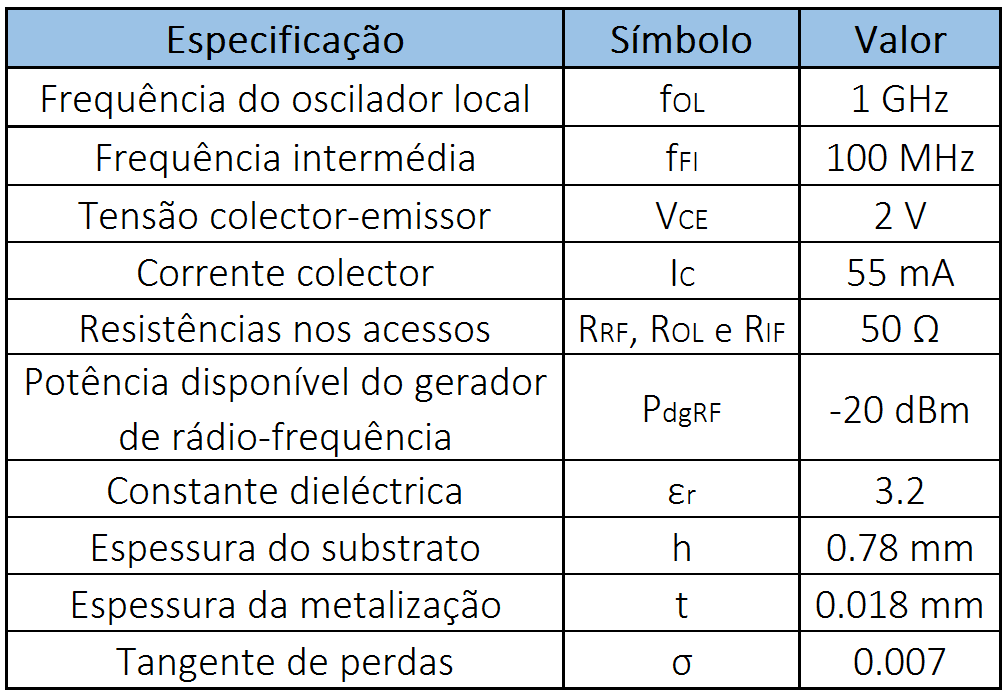
\includegraphics[keepaspectratio=true, scale=0.35]{teoricas/table1}
\label{tab:car}
\end{table}

De notar que o valor da espessura do substrato foi modificado de 0.78 mm para 0.35 mm, com o objectivo de garantir propagação transversal nas linhas de microfita, ou seja, garantir que estas têm um comprimento maior que a largura. \unsure{isto e para manter?}

\section{Misturador com oscilador local na base}

\subsection{a) Dimensionamento dos componentes}

Numa primeira fase considera-se o circuito da Figura TAL sem filtro de frequência intermédia (FI) e sem malha de adaptação.

\paragraph{PFR pretendido} \hspace{0pt} 

Pretende-se determinar os valores das tensões de polarização $V_{BB}$ e $V_{CC}$. Tal como referido na Tabela \ref{tab:car}, as características do ponto de funcionamento em repouso (PFR) já estão pré-definidas, como o valor de $V_{CE}$ e $I_{C}$. Assim, através de uma \texttt{I\_Probe} e fazendo variar os valores de tensão que se pretende calcular, e possível obter os valores que estas tensões assumem quando se obtém o ponto de funcionamento em repouso desejado. Assim,

\vspace{-3mm}
\begin{equation}
\centering
V_{BB} = 0.72~\text{V} ~ e ~ V_{CC} = 2~\text{V}.
\end{equation}

\vspace{1mm} 
Para determinar os valores referidos anteriormente, a simulação foi realizada com componentes ideais, nomeadamente as bobines de bloqueio e os condensadores de desacoplamento, no entanto, estes terão de ser dimensionados de modo a que os elementos reais realizem as suas funções sem perturbar o funcionamento do circuito.

Recorrendo às equações \ref{eq:cond_cap} e \ref{eq:cond_ind}, é possível calcular os valores dos condensadores e bobines que respeitem as condições referentes às impedâncias características das linhas de transmissão.

No caso do condensador de desacoplamento, $C_{D}$, o seu valor tem de cumprir a condição especificada na equação \ref{eq:cond_cap}, pois sabe-se que a impedância dos condensadores de desacoplamento deve ser bastante inferior à impedância característica das linhas de transmissão. 

\vspace{-3mm}
\begin{equation}
	\lvert Z_C \rvert = \frac{1}{w_{0} C_{D}} << Z_0 \hspace{2mm} \rightarrow \hspace{2mm} C_{D} > \frac{1}{w_{0}Z_0 \times 0.1} \hspace{2mm} \rightarrow \hspace{2mm} C_{D} > \dfrac{1}{5 \times w_{0}}.
	\label{eq:cond_cap}
\end{equation}

\vspace{1mm}
No caso da bobine de bloqueio, $L_{CHK}$, o seu valor tem de cumprir a condição especificada na equação \ref{eq:cond_ind}, pois sabe-se que a impedância das bobines de bloqueio deve ser bastante superior à impedância característica das linhas de transmissão.  

\vspace{-3mm}
\begin{equation}
	\lvert Z_L \rvert = w_{0} L_{CHK} >> Z_0 \hspace{2mm} \rightarrow \hspace{2mm} L_{CHK} > \frac{Z_0 \times 10}{w_{0}} \hspace{2mm} \rightarrow \hspace{2mm} L_{CHK} > \frac{500}{w_{0}}.
	\label{eq:cond_ind}
\end{equation}

\vspace{1mm}

Assim, os valores obtidos para os componentes a dimensionar são:

\vspace{-3mm}
\begin{equation}
\centering
C_{1} > \frac{1}{5 \times 2 \pi \times 1 \times 10^{9}} = 31.83~\text{pF};~ C_{2} > \frac{1}{5 \times 2\pi \times 100 \times 10^{6}} = 318.3~\text{pF}; 
\end{equation}
\vspace{-3mm}
\begin{equation}
\centering
L_{CH1} > \frac{500}{2\pi \times 1 \times 10^{9}} = 79.58~\text{nH};~L_{CH2} > \frac{500}{2\pi \times 100 \times 10^{6}} = 795.8~\text{nH}.
\end{equation}

\vspace{2mm}
As condições dos valores do condensador $ C_{1} $ e da bobine $ L_{CH1} $ foram calculadas com um valor de frequência de 100 MHz, correspondente à frequência $f_{FI}$, pois é esta a frequência esperada nesse ramo do circuito. Já as condições correspondentes ao condensador $ C_{2} $ e à bobine $ L_{CH2} $ foram calculadas com um valor de frequência de 1 GHz, correspondente à frequência $ f_{OL} $, pois é esta a frequência esperada nesse ramo do circuito. Foram escolhidos valores para estes componentes que correspondam a valores de mercado, tal como se pode consultar	 na Tabela \ref{tab:cap_ind}.

\begin{table}[h]
	\centering
	\caption{Valores utilizados para os condensadores de desacoplamento e bobines de bloqueio.}
	\vspace{-1.5mm}
	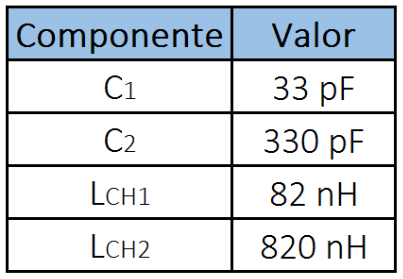
\includegraphics[keepaspectratio=true, scale=0.35]{teoricas/componentes}
	\label{tab:cap_ind}
\end{table}

\todo{e necessario descrever as funcoes dos componentes}

\paragraph{Ganho de transdução de conversão} \hspace{0pt} 

O circuito, agora com elementos reais, pode ser simulado. de acordo com o que se pode observar na Figura \ref{fig:Circuito_0}.

\begin{figure}[h]
\centering
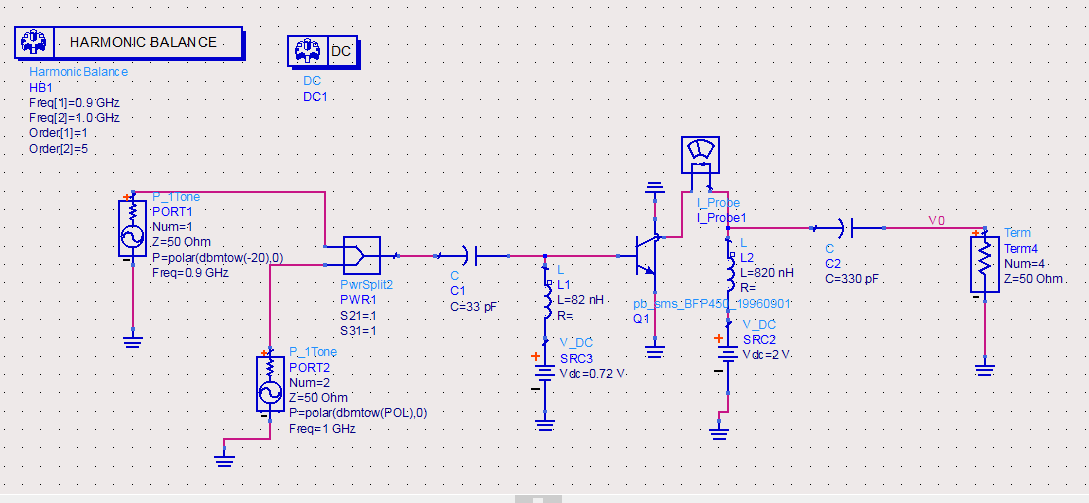
\includegraphics[keepaspectratio=true, scale=0.45]{exps/Circuito_2c}
\vspace{-0.5em}
\caption{Circuito inicial com bobines e condensadores reais.}
\vspace{-0.8em}
\label{fig:Circuito_0}
\end{figure}

Simulando o circuito de forma a obter o gráfico do ganho de transdução de conversão deste circuito vem:

\begin{figure}[h]
\centering
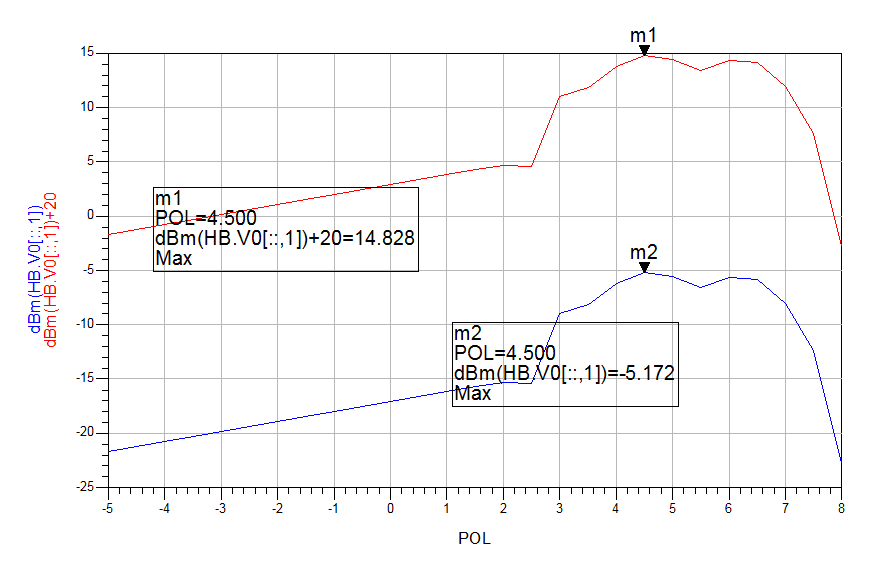
\includegraphics[keepaspectratio=true, scale=0.45]{exps/GT_0}
\vspace{-0.5em}
\caption{Gráfico do ganho de transdução de conversão em função de $ P_{\text{OLDISP}\left(\omega_{OL}\right)} $}.
\vspace{-0.8em}
\label{fig:GT_0}
\end{figure}

Ao observar a Figura \ref{fig:GT_0} é possível determinar o valor de $ P_{\text{OLDISP}\left(\omega_{OL}\right)} $ para qual o ganho de transdução de conversão é máximo, ou seja, -4.5 dBm.

\paragraph{Espectros de potência} \hspace{0pt} 

Usando o mesmo circuito da Figura \ref{fig:Circuito_0} foi possível obter o gráfico com os espectros de potência na Figura \ref{fig:EP_0}.

\begin{figure}[h]
\centering
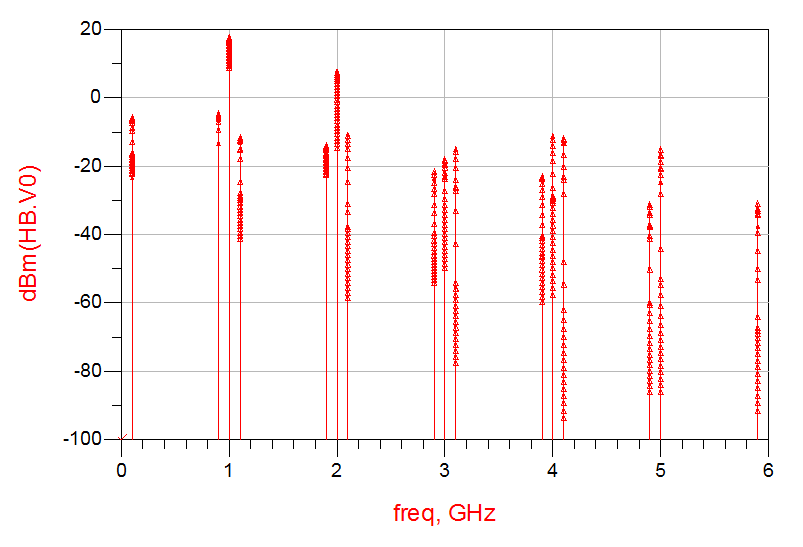
\includegraphics[keepaspectratio=true, scale=0.45]{exps/EP_0}
\vspace{-0.5em}
\caption{Gráfico do ganho de transcondução de conversão em função de $ P_{OLDISP(\omega_{OL})} $.}
\vspace{-0.8em}
\label{fig:EP_0}
\end{figure}

Ao observar a Figura \ref{fig:EP_0} 

\todo{fazer os espectros}

\paragraph{Ganho de conversão} \hspace{0pt} 

\todo{fazer o ganho de conversão}

\paragraph{Filtro de FI}

Teremos como referência o valor da frequência $ f_{FI} $, ou seja, $ \omega_{0}=2\pi f_{FI} $ e um factor de qualidade do filtro de 10. 

\begin{equation}
\omega_{0}=\frac{1}{\sqrt{C_{0}L_{0}}} ~ e ~ B=\frac{1}{R_{FI}C_{0}} ~ e ~ Q=\frac{\omega_{0}}{B}.
\label{eq:filtro_0}
\end{equation}

Tendo em conta as expressões na Equação \ref{eq:filtro_0}, é possível determinar os componentes que compõem o filtro.

\paragraph{Concretização do amplificador em tecnologia de microfita}

Nesta segunda fase o circuito do amplificador será todo projectado com a tecnologia de microfita e irá ser projectado um \textit{layout} do circuito.

\subsubsection{a) Introdução de elementos que simulam descontinuidades nas linhas}

Em primeiro lugar, substitui-se ambas as bobines e as suas fontes de tensão pelo bloco demonstrado na Figura , isto de modo a utilizar tecnologia de microfita para simular as bobines. 


O elemento \texttt{MLIN} com o nome de \texttt{TL7} representado na Figura  tem dimensões obtidas através da ferramenta \texttt{LineCalc} já antes utilizada, no entanto, como argumentos, recebe impedância característica de $100 \Omega$ e comprimento eléctrico de $90^{\circ}$. O elemento \texttt{MLIN} com o nome de \texttt{TL8} tem dimensões calculadas através do mesmo método, no entanto, recebe como impedância característica um valor de $30 \Omega$. Esta alteração no cálculo das dimensões dos elementos \texttt{MLIN} irá causar uma diferença na largura de ambos, sendo necessário usar um elemento \texttt{MSTEP} que tem como objectivo servir de ``adaptador'' para a diferença das larguras entre os canais.

Em relação às quatro descontinuidades criadas nos nós dos circuitos serão usados elementos \texttt{MTEE} que terão como função criar uma junção entre três canais e também, se necessário, adaptar as suas larguras. O resultado destas modificações no circuito do amplificador podem ser observadas na Figura.

Após ter o circuito projectado é possível observar os parâmetros S, Figura , que caracterizam o amplificador.


Como se pode observar, os resultados obtidos não são satisfatórios, os valores máximos/mínimos não se encontram centrados na frequência desejada e não apresentam valores tão próximos do esperado. Assim, foi utilizada a ferramenta \texttt{TUNE} nos comprimentos dos elementos \texttt{MLIN} com o nome de \texttt{TL2}, \texttt{TL1}, \texttt{TL4}, \texttt{TL5}, \texttt{TL7}, \texttt{TL10}, \texttt{TL6} e \texttt{TL11} representados na Figura , onde foi possível obter as características representadas na Figura.


Como se pode observar na Figura , o parâmetro de estabilidade para 22 GHz apresenta um valor que garante a estabilidade incondicional do amplificador para 22GHz. Como se pode observar, apenas se pode garantir a estabilidade incondicional numa banda que vai de aproximadamente 15 GHz a 30 GHz. No entando, foi realizada uma nova simulação para determinar a estabilidade do amplificador em banda larga, que pode ser vista na Figura. 

Como se pode observar na Carta de Smith, pode-se concluir que quando carregado com 50$\Omega$, garante-se a estabilidade do circuito em banda larga (10 GHz a 30 GHz). Isto verifica-se pois os parâmetros $S_{11}$ e $S_{22}$ (correspondentes às circunferências de estabilidade) encontram-se contidos no interior da Carta de Smith.


Na Tabela  está uma comparação entre os vários métodos utilizados para projectar o amplificador.


Um dos objectivos do projecto do amplificador, tal como se pode ver na Tabela \ref{tab:car}, era obter um ganho de transdução máximo, tendo sido realizada a adaptação conjugada simultânea com esse objectivo, sendo que o valor esperado para o ganho de transdução seria o apresentado na Tabela \ref{tab:param_S} como MAG. Como se pode observar, o valor obtido é bastante próximo e apresenta uma diferença de $0.257$ dB, que é causada pelas perdas nas microfitas. Não existia qualquer tipo de especificação em relação ao factor de ruído, no entanto, em relação ao amplificador com linhas ideais, o projecto final do amplificador (amplificador sem descontinuidades pós-\textit{tune}) apresenta um valor mais satisfatório, diminuindo ainda mais a importância da diferença entre o ganho de transdução dos dois amplificadores (linhas ideais e projecto final).

Os valores de ambos os factores de reflexão são muito inferiores em módulo em relação aos simulados no amplificador com linhas ideais. Isto acontece pois o objectivo durante a utilização da ferramenta de optimização (\texttt{TUNE}) era maximizar o valor do ganho de transdução, manter o máximo do ganho de transdução e os mínimos de ambos os factores de reflexão centrados na frequência 22 GHz, sem comprometer em demasia os valores mínimos de ambos os factores de reflexão. É preciso ter em conta que, por exemplo, obter um factor de reflexão à entrada com o valor de -79 dB e à saída com um valor de -10 dB é muito menos favorável que ter ambos os factores de reflexão a -15 dB. Assim, foi definido como valor mínimo aceitável para ambos os factores de reflexão -15 dB, no entanto, enquanto o processo de optimização avançava, a precisão do \texttt{TUNE} era aumentada progressivamente. Foram então obtidos os valores apresentados na Tabela.

\subsubsection{b) Substituição do transístor e condensadores}

Em primeiro lugar, tem de se determinar as dimensões dos condensadores e, sabendo que estes têm um valor de 39 pF, foi necessário recorrer a uma \textit{datasheet} de condensadores com esse valor, sendo escolhida a do elemento \texttt{KEMET Part Number: C0402C390J5GACTU}. As suas dimensões podem ser consultadas na Figura, e são calculados na Equação .


\vspace{-1mm}
Pode-se então determinar a dimensão dos elementos \texttt{MGAP} a utilizar para substituir os condensadores. No entanto, como os condensadores têm uma largura diferente da do canal onde estão a ser inseridos, é necessário usar \texttt{MSTEP's} para adaptar os condensadores ao canal.

Para substituir o transístor pelo elemento \texttt{MGAP} tem de se calcular as dimensões de largura e comprimento a utilizar. Ao se consultar o \textit{datasheet} do transístor é possível concluir que o encapsulamento tem $1.76$ mm, pelo que é necessário uma dimensão S do elemento \texttt{MGAP} ligeiramente superior, diga-se $2.5$ mm. Em relação à largura do \texttt{MGAP}, esta tem de coincidir com o tamanho dos \textit{pins} da \textit{gate} e do \textit{dreno} do transístor, $0.51$ mm. Mais uma vez, como a dimensão da largura do \texttt{MGAP} não é igual à do canal em que este será inserido, foram usados elementos\texttt{MSTEP} para adaptar o canal.

O circuito que resulta destas substituições dos condensadores e transístores pode ser observado na Figura .


Ao ter o circuito totalmente projectado, é possível usar a ferramenta \texttt{layout} do ADS para construir o \textit{layout} do circuito, que pode ser observado na Figura.


O \textit{layout} obtido é satisfatório visto que apresenta as microfitas projectadas, e os espaços destinados aos condensadores e transistor com as dimensões projectadas.

\section{Conclusões}

Foi projectado e simulado um amplificador preparado para trabalhar na frequência de 22 GHz utilizando a tecnologia de microfita. Em análise à Tabela pode-se concluir que as especificações da Tabela \ref{tab:car} foram alcançadas, desde o ponto de funcionamento em repouso, ao ganho de transdução.

Ao utilizar o ADS e as suas ferramentas, concluiu-se que é um programa de grande utilidade, e que o seu potencial é enorme para projectar circuitos que trabalhem em altas frequências.

\end{document}